\documentclass{article}
\usepackage[utf8]{inputenc}

\title{481 - Homework 7}
\author{Victor Zhang}
\date{October 19, 2020}

\usepackage[utf8]{inputenc}
\usepackage{amsmath}
\usepackage{amsfonts}
\usepackage{natbib}
\usepackage{graphicx}
% \usepackage{changepage}
\usepackage{amssymb}
\usepackage{xfrac}
% \usepackage{bm}
% \usepackage{empheq}
\usepackage{tikz}

\newcommand{\contra}{\raisebox{\depth}{\#}}

\newenvironment{myindentpar}[1]
  {\begin{list}{}
          {\setlength{\leftmargin}{#1}
          \setlength{\rightmargin}{#1}}

          \item[]
  }
  {\end{list}}

\pagestyle{empty}

\begin{document}

\maketitle
% \begin{center}
% {\huge Econ 482 \hspace{0.5cm} HW 3}\
% {\Large \textbf{Victor Zhang}}\
% {\Large February 18, 2020}
% \end{center}

\section*{8.33}
Put $X \sim t_n$. Since the distribution function of $X$ is even, $E[X] = 0$, assuming $n \geq 2$. Since $\mathrm{var}(X) = E[X^2] - E[X]^2$, $\mathrm{var}(X) = E[X^2]$. Now we compute $E[X^2]$. Note $X \sim \frac{Z}{\sqrt{\chi^2_n}/n}$ so $X^2 \sim \frac{\chi^2_1}{\chi^2/n}$. Put $U \sim \chi^2_1$ and $V \sim \chi^2_n$. By definition of $X$, $U$ and $V$ are independent. So we may integrate
\begin{equation*}
\begin{split}
E[X^2] &= \int\limits_0^\infty \int\limits_0^\infty \frac{u}{v/n}f_U(u)f_V(v)\; \mathrm{d}u\; \mathrm{d}v\\
&= \int_0^\infty E[U] \frac{n}{v}f_V(v)\; \mathrm{d}v\\
&= \int_0^\infty \frac{n}{v}f_V(v)\; \mathrm{d}v\\
&= \int_0^\infty \frac{n}{v}f_V(v)\; \mathrm{d}v\\
&= \int_0^\infty \frac{n}{2^{n/2}\Gamma(n/2)}v^{n/2-2}e^{-v/2} \; \mathrm{d}v\\
\end{split}
\end{equation*}
Substituting $v = 2t$,
$$E[X^2] = \frac{n}{2^{n/2-1}\Gamma(n/2)} \int\limits_0^\infty (2t)^{n/2-2}e^{-t}\; \mathrm{d}t = \frac{n}{2\Gamma(n/2)} \int\limits_0^\infty t^{n/2-2}e^{-t}\; \mathrm{d}t$$
We note the integral matches the definition of the gamma function, so in fact
$$E[X^2] = \frac{n\Gamma(n/2 - 1)}{2\Gamma(n/2)} = \frac{n}{2(n/2-1)} = \frac{n}{n-2} \; \Box$$
Alternatively we may recognize $X^2 \sim F(1,n)$ and arrive at the conclusion immediately.

\section*{8.36}
$f_{t_1}(x) = \frac{c}{1+t^2}$, so $t_1$ is exactly the Cauchy distribution $\Box$

\section*{11.1}
$$Pr(0 < \theta < kx) = Pr(x > \frac{\theta}{k}) = \int\limits_{\theta/k}^\infty \frac{1}{\theta}e^{-x/\theta} \; \mathrm{d}x = e^{-1/k} = 1-\alpha$$
Solving yields $k = -\frac{1}{\ln(1-\alpha)}$ $\Box$

\section*{11.2}
\begin{equation*}Pr(0 < \theta < k(x_1+x_2)) = Pr(x_1+x_2 > \frac{\theta}{k}) = 1- \alpha\end{equation*}
\subsection*{11.2.1}

\tikzset{every picture/.style={line width=0.75pt}} %set default line width to 0.75pt        

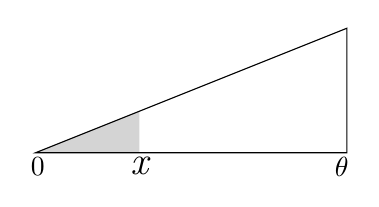
\begin{tikzpicture}[x=0.75pt,y=0.75pt,yscale=-1,xscale=1]
%uncomment if require: \path (0,168); %set diagram left start at 0, and has height of 168

%Shape: Right Triangle [id:dp23247894729782836] 
\draw  [draw opacity=0][fill={rgb, 255:red, 212; green, 212; blue, 212 }  ,fill opacity=1 ] (60,60) -- (10,80) -- (60,80) -- cycle ;
%Shape: Right Triangle [id:dp6579992124182097] 
\draw   (160,20) -- (10,80) -- (160,80) -- cycle ;

% Text Node
\draw (54.5,81) node [anchor=north west][inner sep=0.75pt]  [font=\normalsize] [align=left] {{\Large \textit{x}}};
% Text Node
\draw (153,80.9) node [anchor=north west][inner sep=0.75pt]    {$\theta $};
% Text Node
\draw (6.5,80.9) node [anchor=north west][inner sep=0.75pt]    {$0$};

\end{tikzpicture}

\noindent
Consider the diagram above. Note the grey region has area $\frac{1}{2}\frac{x^2}{\theta^2}$. If region has area $\alpha$, $x = \theta\sqrt{2\alpha}$. Then $\frac{\theta}{k} = \theta\sqrt{2\alpha}$ and $k=\frac{1}{\sqrt{2\alpha}}$ when $\alpha \leq \frac{1}{2}$.

\subsection*{11.2.2}

\tikzset{every picture/.style={line width=0.75pt}} %set default line width to 0.75pt        

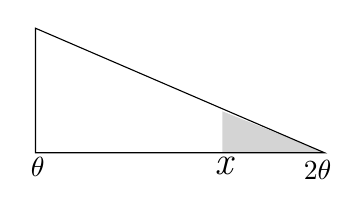
\begin{tikzpicture}[x=0.75pt,y=0.75pt,yscale=-1,xscale=1]
%uncomment if require: \path (0,168); %set diagram left start at 0, and has height of 168

%Shape: Right Triangle [id:dp23247894729782836] 
\draw  [draw opacity=0][fill={rgb, 255:red, 212; green, 212; blue, 212 }  ,fill opacity=1 ] (100,60) -- (150,80) -- (100,80) -- cycle ;
%Shape: Right Triangle [id:dp6579992124182097] 
\draw   (10,20) -- (149.25,80) -- (10,80) -- cycle ;

% Text Node
\draw (95,81) node [anchor=north west][inner sep=0.75pt]  [font=\normalsize] [align=left] {{\Large \textit{x}}};
% Text Node
\draw (138,82.4) node [anchor=north west][inner sep=0.75pt]    {$2\theta $};
% Text Node
\draw (6.5,80.9) node [anchor=north west][inner sep=0.75pt]    {$\theta $};


\end{tikzpicture}

\noindent
Similarly to the previous section, the grey region has area $1-\alpha = \frac{1}{2}\frac{(2\theta-x)^2}{\theta^2}$. Then $k = \frac{1}{2-\sqrt{2(1-\alpha)}}$ when $\alpha > \frac{1}{2}$ $\Box$

\section*{11.3}
We are guaranteed $R < \theta$ so it suffices to find $c$ s.t. $Pr(\theta < cR) = 1-\alpha$.
$$Pr(\theta < cR) = Pr(R > \frac{\theta}{c}) = \int\limits_{\theta/c}^{\theta} \frac{2}{\theta^2}(\theta-R)\; \mathrm{d}R = 1 - \frac{2}{c} + \frac{1}{c^2} = \left(1-\frac{1}{c}\right)^2 = 1-\alpha$$
Thus, $c = \frac{1}{1-\sqrt{1-\alpha}}$ $\Box$

\section*{11.4}
This follows directly from the results of section 11.5, namely that the symmetric confidence interval minimizes the length of the interval.

\section*{11.5}
The following derivation is quoted from (my) solution of quiz 6.
\begin{myindentpar}{1em}
It suffices to show for $p_1+p_2 = \alpha$ that $Z_{p_1}+Z_{p_2}$ is minimized when $p_1=p_2=\frac{\alpha}{2}$. WLOG suppose $p_1 > p_2$, that is, $Z_{p_1} < Z_{p_2}$. Consider $Z_{p_1+\varepsilon} + Z_{p_2-\varepsilon}$ for $\varepsilon > 0$. Since the density of $Z$ is greater at $p_1$ than at $p_2$, it is easy to see that $Z_{p_1+\varepsilon} + Z_{p_2-\varepsilon} > Z_{p_1}+Z_{p_2}$. Similarly, $Z_{p_1-\varepsilon} + Z_{p_2+\varepsilon} < Z_{p_1}+Z_{p_2}$. Thus, if $p_1 > p_2$ we may find some smaller sum by decreasing $p_1$ by $\varepsilon$. Likewise, if $p_1 < p_2$, we may find some smaller sum by increasing $p_1$ by $\varepsilon$. Thus, $Z_{p_1}+Z_{p_2}$ is minimized when $p_1 = p_2 = \frac{\alpha}{2}$ and we are done $\Box$
\end{myindentpar}

\section*{11.6}
For large $n$ we may say by CLT that $\overline{x} \sim N(\mu,\sigma^2/n)$. Then $\frac{\overline{x}-\mu}{\sigma/\sqrt{n}} \sim Z$. By confidence interval for the standard normal, $Pr(-z_{\alpha/2} < \frac{\overline{x}-\mu}{\sigma/\sqrt{n}} < z_{\alpha/2}) = 1-\alpha$. Then $e = z_{\alpha/2}\frac{\sigma}{\sqrt{n}}$ and $n = \left[z_{\alpha/2}\frac{\sigma}{e}\right]^2$ $\Box$

\end{document}

% List of tex snippets:
%   - tex-header (this)
%   - R      --> \mathbb{R}
%   - Z      --> \mathbb{Z}
%   - B      --> \mathcal{B}
%   - E      --> \mathcal{E}
%   - M      --> \mathcal{M}
%   - m      --> \mathfrak{m}({#1})
%   - normlp --> \norm{{#1}}_{L^{{#2}}}
